\documentclass{article}

\usepackage{graphicx} % Required for inserting images
\usepackage[left=1in,right=1in,top=1in,bottom=1in]{geometry}
\usepackage{amsmath}
\usepackage{amsthm} %proof environment
\usepackage{amssymb}
\usepackage{amsfonts}
\usepackage{enumitem} %nice lists
\usepackage{verbatim} %useful for something 
\usepackage{xcolor}
\usepackage{setspace}
\usepackage{titlesec}
\usepackage{blindtext} % I have no idea what this is 
\usepackage{caption}  % need this for unnumbered captions/figures
\usepackage{natbib}
\usepackage{tikz}
\usepackage{hyperref}

\titleformat{\section}{\bfseries\Large}{Problem \thesection:}{5pt}{}
\titleformat{\subsection}{\bfseries\large}{Subproblem \thesubsection:}{5pt}{}

\begin{document}

\title{AM 160 - SciML:}
\author{Dante Buhl}


\newcommand{\wrms}{w_{\text{rms}}}
\newcommand{\bs}[1]{\boldsymbol{#1}}
\newcommand{\tb}[1]{\textbf{#1}}
\newcommand{\bmp}[1]{\begin{minipage}{#1\textwidth}}
\newcommand{\emp}{\end{minipage}}
\newcommand{\R}{\mathbb{R}}
\newcommand{\C}{\mathbb{C}}
\newcommand{\N}{\mathcal{N}}
\newcommand{\K}{\bs{\mathrm{K}}}
\newcommand{\m}{\bs{\mu}_*}
\newcommand{\s}{\bs{\Sigma}_*}
\newcommand{\dt}{\Delta t}
\newcommand{\dx}{\Delta x}
\newcommand{\tr}[1]{\text{Tr}(#1)}
\newcommand{\Tr}[1]{\text{Tr}(#1)}
\newcommand{\Div}{\nabla \cdot}
\renewcommand{\div}{\nabla \cdot}
\newcommand{\Curl}{\nabla \times}
\newcommand{\Grad}{\nabla}
\newcommand{\grad}{\nabla}
\newcommand{\grads}{\nabla_s}
\newcommand{\gradf}{\nabla_f}
\newcommand{\xs}{x_s}
\newcommand{\xf}{x_f}
\newcommand{\ts}{t_s}
\newcommand{\tf}{t_f}
\newcommand{\pt}{\partial t}
\newcommand{\pz}{\partial z}
\newcommand{\uvec}{\bs{u}}
\newcommand{\F}{\bs{F}}
\newcommand{\T}{\tilde{T}}
\newcommand{\ez}{\bs{e}_z}
\newcommand{\ex}{\bs{e}_x}
\newcommand{\ey}{\bs{e}_y}
\newcommand{\eo}{\bs{e}_{\bs{\Omega}}}
\newcommand{\ppt}[1]{\frac{\partial #1}{\partial t}}
\newcommand{\DDt}[1]{\frac{D #1}{D t}}
\newcommand{\ppts}[1]{\frac{\partial #1}{\partial t_s}}
\newcommand{\pptf}[1]{\frac{\partial #1}{\partial t_f}}
\newcommand{\ppz}[1]{\frac{\partial #1}{\partial z}}
\newcommand{\ddz}[1]{\frac{d #1}{d z}}
\newcommand{\ppzetas}[1]{\frac{\partial^2 #1}{\partial \zeta^2}}
\newcommand{\ppzs}[1]{\frac{\partial #1}{\partial z_s}}
\newcommand{\ppzf}[1]{\frac{\partial #1}{\partial z_f}}
\newcommand{\ppx}[1]{\frac{\partial #1}{\partial x}}
\newcommand{\ppxi}[1]{\frac{\partial #1}{\partial x_i}}
\newcommand{\ppxj}[1]{\frac{\partial #1}{\partial x_j}}
\newcommand{\ppy}[1]{\frac{\partial #1}{\partial y}}
\newcommand{\ppzeta}[1]{\frac{\partial #1}{\partial \zeta}}


\maketitle 
% This line removes the automatic indentation on new paragraphs
\setlength{\parindent}{0pt}
\doublespacing

\section{}

\subsection{}
Show that $\Theta = A^{\dagger}y$ is the solution such that $||\Theta||_2$ is
the minimum out of all the infinite solutions to $y = A\Theta$. Consider $A \in
\R^{n\times p}$ where $p\gg n$. 


\begin{proof}
    We begin by writing the SVD of $A$ which is part of the construction of the
    psuedoinverse $A^{\dagger}$. 
    \begin{gather*}
        A = U\Sigma V^*\\
        A^{\dagger} = V\Sigma^{-1}U^*
    \end{gather*}
    where $U$ and $V$ are unitary matrices, and $\Sigma^{-1}$ is the transpose of $\Sigma$ containing the reciprocal
    of each singular value (in order) along the diagonal, i.e. 
    \begin{gather*}
        \Sigma^{-1} = \left[\begin{array}{c c c}
                            1/\sigma_1 & & \bs{0}  \\
                             &\ddots &  \\
                            \bs{0} & & 1/\sigma_n \\
                            \hline &\bs{0}&
                            \end{array}\right]
    \end{gather*}
    Next we need to understand why $\Theta$ in this context has infinitely many
    solutions. Let us assume that $A$ is rank $n$. The implication is that there
    are at most $n$ basis vectors in $\R^{p}$ which are not in the null space of
    the transformation $A$. We can write $\Theta$ as a linear combination
    of basis vectors which span $\R^{p}$
    \begin{gather*}
        \Theta = c_1v_1 + \ldots + c_nv_n + \ldots + c_pv_p
    \end{gather*}
    Notice though, however, that only $n$ of these vectors are in the kernel of
    $A$ (and let us assume it is the first $n$ vectors for convenience). We have
    then that all vectors $v_{n+1}, \ldots, v_{p}$ in the linear combination of
    $\Theta$ do not affect the solution. Therefore, an infinite number of
    solutions $\Theta$ can be created by adding the linear combination of
    $v_{n+1}, \ldots, v_p$ to any solution of $y = A\Theta$. 


    In order to see why the psuedouinverse $A^{\dagger}$ yields the minimum
    solution is because it projects the $p$ dimension problem into a $n$
    dimension problem, i.e.
    \begin{gather*}
        y = A\Theta \\
        y = U\Sigma V^*\Theta\\
        y = UC
    \end{gather*}
    where $C$ is an $n\times1$ vector which literally contains the coefficients
    of the linear combination for the first $n$ basis vectors of $\Theta$ scaled
    by their corresponding singular value $\sigma_i$, i.e. $C_i = c_i\sigma_i$. 

    Finally, we solve for $C$ (which has one unique solution since $U$ is full
    rank) using the inverse of $U$ which exists since $U$ is
    unitary. 
    \begin{gather*}
        C = U^*y
    \end{gather*}
    Notice that this constructs $\Theta$ out of the minimum number of basis
    vectors in order to span $\R^{n}$ that is, for any $y$ given. Then looking at
    the 2-norm of $\Theta$ we have, 
    \begin{align*}
        ||\Theta||_2 &= ||c_1v_1||_2 + \ldots + ||c_nv_n||_2\\
         &= |c_1|||v_1||_2 + \ldots + |c_n|||v_n||_2\\
         &= |c_1| + \ldots + |c_n|
    \end{align*}
    where we can decompose the 2-norm in this way because the basis vectors
    $v_i$ are orthogonal to each other in the 2-norm. Notice that the addition
    of any additional $\R^{p}$ basis vectors will only increase the 2-norm of
    $\Theta$. We conclude then that solving for $\Theta$ using the psuedoinverse
    of $A$ yields $\Theta$ such that the 2-norm of $\Theta$ is the minimum out
    of all possible $\Theta$ which solve $y=A\Theta$. 

    The proof at the end of Lecture Notes 4, essentially demonstrates this as
    well. The basis of the proof is that any of the infinitely many solutions
    can be constructed as
    \begin{gather*}
        \Theta = \Theta' + \Theta^*
    \end{gather*}
    and proceeds to show that $\left<\Theta', \Theta^*\right> = 0$, i.e. that
    $\Theta'$ is orthogonal to $\Theta^*$. As I have shown earlier, the infinite
    solutions for $\Theta$ arise by introducing a linear combination of the
    vectors in the Null space of $A$, i.e.
    \begin{gather*}
        \Theta = \Theta^* + c_{n+1}v_{n+1} + \ldots + c_pv_p\\
        \Theta' = c_{n+1}v_{n+1} + \ldots + c_pv_p
    \end{gather*}
    Finally, since $\Theta'$ is constructed of basis vectors of $\R^p$ all of
    which are orthogonal to $\Theta^*$, we have that
    $\left<\Theta',\Theta^*\right> = 0$. The rest of the proof in the lecture
    notes holds (assuming $\Theta' \ne 0$), 
    \begin{align*}
        \left<\Theta, \Theta\right> &=
        \left<\Theta'+\Theta^*,\Theta'+\Theta^*\right>\\
        &= \Theta'^T\Theta' + \Theta'^T\Theta^* + \Theta^{*T}\Theta' +
        \Theta^{*T}\Theta^*\\
        &= \left<\Theta',\Theta'\right> + 2\left<\Theta',\Theta^*\right> +
        \left<\Theta^*, \Theta^*\right>\\
        &= \left<\Theta',\Theta'\right> + \left<\Theta^*,\Theta^*\right> > \left<\Theta^*,\Theta^*\right>
    \end{align*}
    where both $\left<\Theta', \Theta'\right>$ and $\left<\Theta^*,
    \Theta^*\right>$ are semi-positive definite terms. Therefore, we have that
    $\Theta^* = \text{argmin}_{y=A\Theta}||\Theta||_2$. 

\end{proof}

\subsection{}

\begin{figure}[ht]
    \centering
    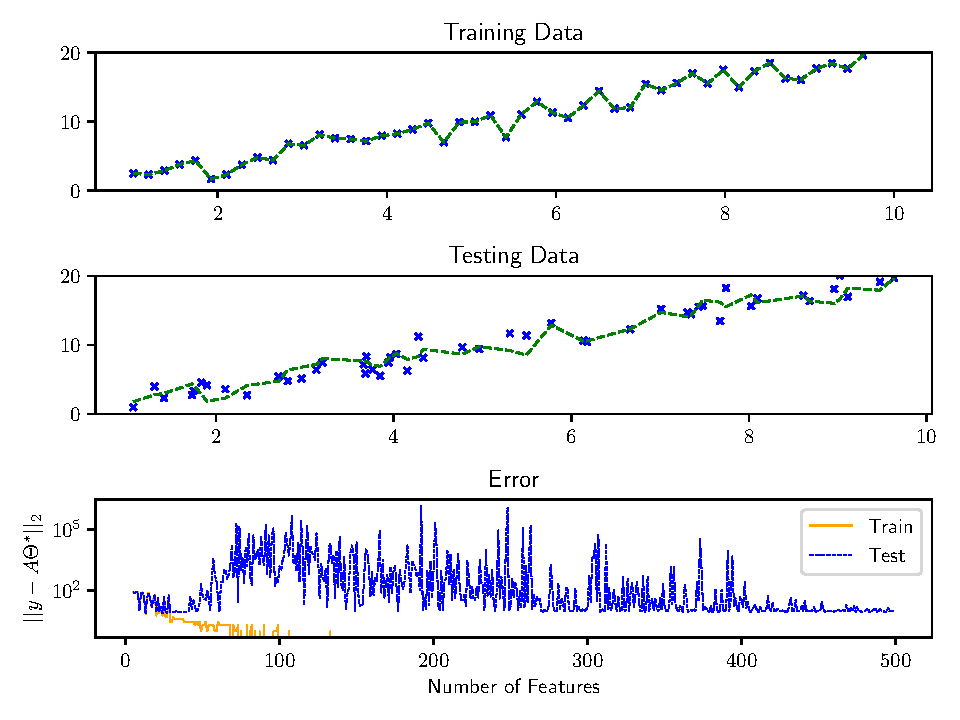
\includegraphics[width=\textwidth]{hw1s2.pdf}
    \caption{Training, Test, and Error data from the linear regression posed in
    subproblem 2. The training and test data plots show how well the linear
    regression fits to the data given in both the training and testing cases for
    $p=500$. The error plot shows both the training and testing error as a
    function of the number of features $p$, in order to demonstrate double
    descent.}
    \label{fig:s2}
\end{figure}

In order to demonstrate double descent using a random Fourier feature matrix
$A$, we perform a linera regression for the function, 
\begin{gather}
    y = 2x + \cos(25x) + r
    \label{eq:s2}
\end{gather}
where $r$ is gaussian noise sampled from the standard normal distribution $\mathcal{N}(0,1)$.
Since the purpose of the linear regression 
\begin{gather*}
    y = A\Theta
\end{gather*}
is to build a fourier cosine series which interpolates \eqref{eq:s2}, where the
vector $\Theta$ is the coefficient vector for each random fourier mode
$\phi_i(x) = \cos(2\pi w_ix)$, where $w_i \sim \mathcal{N}(0,1)$. For my work
specifically, I have chosen to use 50 data points for each of the training and
the test set on the domain $x \in [1,10]$. It is necesary for both data sets to
be taken from the same domain, as fourier series usually only interpolate
functions in a finite domain. 

As a result, the number of features used in this regression problem will be
start at 5 features ($p \ll n$), and end at 500 features ($p \gg n$) with
increments of 1. Notice
that depending on the type of system being solved (overdetermined v.s.
underdetermined) the method of obtaining $\Theta$ will change from a least
squares solution to a psuedoinverse solution, i.e.
\begin{gather*}
    \Theta = \text{argmin}_{y = A\Theta} ||y - A\Theta||_2, \quad p < n\\
    \Theta = A^{\dagger}y, \quad p \ge n
\end{gather*}
Thus, we obtain the error v.s. feature plot that is seen in figure \ref{fig:s2},
where there appears to be a double descent which settles to the minimum test
error near $p \approx 400$. Note that the minimum test error seems to settle at
$10^1$ which seems natural due to the noise in the data sets which is of $O(10^0)$,
and then scaled by the number of test points which is of order $O(10^1)$, hence
obtaining an average error for the whole data set of $O(10^1)$. 

\end{document}
